%! TEX root = ../../../main.tex

\section{Versioning}%
\label{sec:Versioning}

\subsection{The Need for Good Versioning Conventions}%
\label{sub:The_Need_for_Good_Versioning_Conventions}
Unlike in the monolithic architecture, a continuously deployed microservice
architecture is comprised of many components that each have their own version.
Hence it has to be decided case by case which versioning scheme best fits each
microservice. Further, as many microservices provide some kind of \ac{API}
(mostly \ac{REST}) some form of versioning has to be used. Without versioning,
the application implementing the \ac{API} would always consume the latest
version of the microservice. This implies that any non-backward-compatible
update to the microservice would break all client implementations of the
microservice's \ac{API}. Not only is the client able to pin its implementation
to a specific \ac{API} version. The client is further able to select any
version of a resource that best fits its implementation. In addition, a good
versioning scheme allows developers to quickly assess whether a new version
breaks the service's backward-compatibility. Lastly, microservice do not only
provide services to other microservices. E.g.\ a \textit{frontend} microservice
directly serves the end user. Hence the versioning scheme used in such a
microservice also serves a communicative purpose.

\subsection{Versioning in a Conventions Microservice Environment}%
\label{sub:Versioning_in_a_Microservice_Environment}
Chapter~\ref{sub:Versioning} already introduced the two main versioning schemes
\textit{SemVer} and \textit{CalVer}. As microservices mostly provide their
\ac{API} through the \ac{REST} paradigm, the chapter also presented the three
main possibilities to version a \ac{REST} \ac{API}.

Based on this theoretical foundation, it is the aim to develop a model that
shows how a microservice can be versioned. In addition, it is the goal to
define a process that helps developers to choose the best versioning model for
their given application.

\subsubsection{Versioning Monoliths vs.\ Microservices}%
\label{ssub:Versioning Monoliths_vs_Microservices}

It might seem like that monolithic and microservice applications
follow the same conventions in regards to versioning; at least both application
types are versioned in some form. In addition their code base is stored and
tracked in some form of \ac{VCS}. However they have to be handled quite
differently. Due to their high deployment complexity a microservice
architecture is still primarily employed in the cloud applications. There are a
few ways the microservice architecture can be brought to desktop software.
However due to the definitions of microservices this thesis explored to far,
the upcoming section will only focus on microservice applications that are
deployed in the cloud. In that case, two possible ways of distribution prevail:
distribution as a \ac{SaaS} product or as a software package (e.g.\ in form of
a Helm chart) in the customers cloud environment. In the case of a \ac{SaaS}
solution, the user never interacts with the installation, configuration and
upgrade process. Given the application is deployed by the user inside their
cloud environment, only the version number of the complete software package is
of interest. Even though a microservice architecture is made up of a set of
microservices, the only component a user, in this case an administrator
deploying the application, ever touches is the microservice architecture's
package (e.g.\ a helm chart). Narrowing it further down, this thesis will only
focus on cloud applications that are deployed as part of a \ac{SaaS} product
because of the interest in a continuously deployed microservice architecture.
Yet it is feasible to bring continuous deployment to self-hosted microservice
architectures, this is out of this thesis' scope. From a microservice
architecture developer's perspective, the source code of each microservice is
managed in separate repository inside a \ac{VCS}. This introduces complexity
but also brings the advantage of distinct build configurations if these are
stored in configuration files next to the service's code.

Now that the properties of monolithic and microservice architecture versioning
are recorded, the question of which versioning scheme best fits a microservice
architecture can be addressed. In order to do so, microservices can be divided
into two categories: \textit{Human Interaction} and \textit{Machine
Interaction}. A microservice can be classified in the Human Interaction
category if it mainly used by humans. This is e.g.\ the case for frontend
microservices and other \textit{consuming} parts. On the other hand, a
microservice can be classified in the Machine Interacting category whenever it
mainly talks to other machines or its functionality is integrated in other
microservices in a library like fashion. Such services can also be considered
to be \textit{producing} parts.

\LTXtable{\textwidth}{tables/versioning_machine_human.tex}

Table \ref{tab:versioning_machine_human} shows a selected set of properties
that is required for versioning a microservice. It groups the requirements into
the two microservice categories \textit{Human Interaction} and \textit{Machine
Interaction}. It can be concluded that the versioning of \textit{consuming}
services mainly serves a communicative purpose whereas versioning in
\textit{producing} services plays a technical role. Hence it can be argued that
for microservices which are mainly in direct contact with humans, the version
number is an indicator for features. Thus e.g.\ version 16 of a frontend might
introduce a feature that gives the user more editing capabilities. This added
value can then be clearly communicated using the release's version number.

In a microservice environment these four components can be identified to
receive version numbers (in reverse order of atomicity):

\begin{itemize}
  \item Packaged software (e.g.\ Helm charts)
  \item Container images
  \item Software (e.g.\ Node.js projects)
  \item \acp{API}
\end{itemize}

So far, this section already explored the general issues related to versioning
a microservice. The requirement however demands that the microservices are also
continuously deployed. Despite the fact that an automated build and deployment
process can reduce the workload of a developer and administrator, it introduces
an additional facet of complexity. Whenever a microservice is continuously
built and deployed, it has to be decided who has to bump the version number.
Schemes like SemVer require manual version bumping whereas date-based schemas
like CalVer can be incremented without manual intervention. The reason why
SemVer requires input by a developer is that with each version bump the type of
version increase has to be determined. Each time the version in incremented
these three questions have to be asked:

\begin{itemize}
  \item Does this update only introduce fixes?
  \item Does this update include any new features?
  \item Does this update break the software's backward compatibility?
\end{itemize}

According to the answers to these questions, only the correct part of the
version number has to be modified. The rules for when to update which part of a
SemVer version number are already discussed in chapter~\ref{ssub:SemVer}. These
question however can not be answered by a \ac{CI} solution that is not able to
able to understand the intricate differences between a e.g.\ backward
compatibility breaking update and a simple bug fix. Hence it can be argued that
a versioning scheme that requires artificial decisions from developers can not
be fully supported by \ac{CI} systems. For each new version, the developers
have to manually write the new version number in the applications
configuration. E.g.\ in case of Node.js application, the \texttt{version} field
inside the \texttt{package.json} file has to be updated.

In contrast, date-based versioning schemes like CalVer can update the version
number without further intervention developers. As already discussed in
chapter~\ref{ssub:Date_Based_Versioning}, in most cases a CalVer version number
only includes the formatted date of the release.
Chapter~\ref{ssub:Continuous_Integration} already stated that any software that
is considered to be stable can be used as a release. Thus the \ac{CI} system
can continuously generate a valid date-based version number and inject it in
the software package. Next to the actual application, the same principles can
be applied to packaged software and container images.

Yet, when it comes to \acp{API}, an exception must me made. As pointed out in
chapter~\ref{ssub:API_Versioning}, the usage of \acp{API} heavily depends on
pinning to specific \ac{API} versions. To do so, a number of tactics were
already discussed. The most common \ac{API} versioning scheme differs from the
SemVer and CalVer schemes. Instead of choosing a version number that consists
of three parts (\texttt{MAJOR.MINOR.PATCH}) or is date-based, \acp{API} only
announce their major version. If the major version changes, a backward
compatibility breaking change was implemented. Like with SemVer this results in
a manual process that requires application developers to determine if an update
is major.

\begin{figure}[H]
\begin{center}
  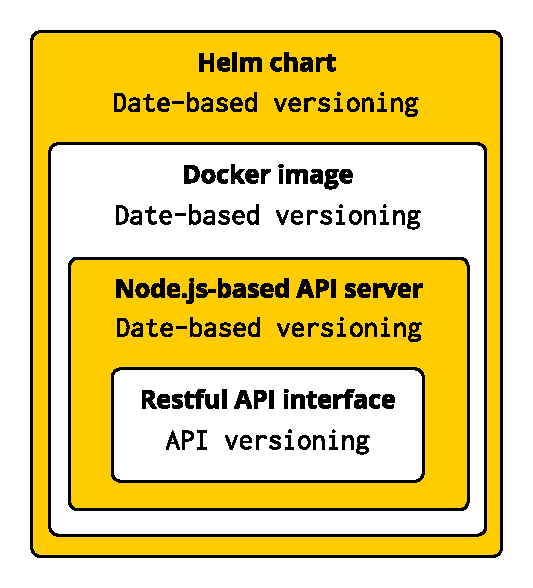
\includegraphics[scale=0.7]{images/figures/version_wrapping.pdf}
\end{center}
\caption{Wrapping inner versioning schemes through levels of abstraction.}%
\label{fig:version_wrapping}
\end{figure}

Even though \acp{API} might need a manual versioning scheme, the abstraction
layers above the actual \ac{REST} interface can be versioned differently. As
shown in figure~\ref{fig:version_wrapping}, the application serving the
\ac{REST} interface, in this case a Node.js application, can use an automated
versioning scheme. This way, the \ac{API}'s manual versioning is masked and a
\ac{CI} system can continuously version the software, the resulting container
image and software package. The inner \ac{API} version is wrapped and thus no
longer relevant to the \ac{CI}/\ac{CD} process.

It can thus be argued that a continuous versioning scheme should be used
whenever possible in order to shift the versioning responsibility from
developers to the \ac{CI} system. Only if the software is dependend on marking
a break in its backward compatibility, the version number should be set
manually using a SemVer-like schema. Hence, both applications consuming as well
as producing data can be versioned using a continuous scheme with this
exception.

\subsubsection{Implementation Using Azure DevOps}%
\label{ssub:Implementation_Using_Azure_DevOps}
The \ac{CI}/\ac{CD} service Azure DevOps can be used to show how a continuous
versioning scheme can be implemented in practise. To dynamically generate and
set date-based version numbers, a number of approaches exist. This section will
explore one possible solution.

In Azure DevOps, each microservice is built using a separate pipeline. One of
the properties that can be set for a pipeline is the \textit{build number
format}. Based on this property, a pipeline's build receives a unique identifier
that can also be accessed during the pipeline's run as a variable. In order to
produce a date-based version in the CalVer format \texttt{YYYYMMDD.MINOR}, the
following build number format \texttt{\$(Date:yyyyMMdd).\$(Rev:r)} can be used.
If set to this value, the first build on e.g. November 24th 2019 produces the
build number \texttt{20191124.1}.

To then access the build number in one of the pipeline's steps, the
\texttt{\$BUILD.BUILDNUMBER} variable can be read. When doing so from a
bash-based shell script, all dots are substituted with underscores. This
results in the variable name \texttt{\$BUILD\textunderscore BUILDNUMBER}.

\begin{listing}[H]
  \begin{minted}{YAML}
steps:
- displayName: 'Inject current build number into package.json'
  script: |
   echo "The current build number is: $BUILD_BUILDNUMBER"
   sed -i "s/1.0.0/1.0.0-$BUILD_BUILDNUMBER/g" package.json
  \end{minted}
  \caption{Injecting a date-based version number into the package.json file of
  a Node.js project using a script-based pipeline task.}%
  \label{listing:version_injection}
\end{listing}

Listing~\ref{listing:version_injection} shows the definition of a Azure DevOps
pipeline task. In it, the \texttt{sed} utility is used to find the version
string \texttt{1.0.0} and replace it with the string
\texttt{1.0.0-\textbf{build number}}. The question of why the string
\texttt{1.0.0} is prefixed to the version string might arise. Node.js demands
that all project use a SemVer version number. However additional information
can be postfixed. The postfix is also consulted when determining the newest
version of a Node.js package; \texttt{1.0.0-20190301.1} $<$
\texttt{1.0.0-20190301.2} $<$ \texttt{1.0.0-20200301.1}. Using this approach, a
Node.js project can take advantage of dynamic version numbers while preserving
the SemVer format.

Next to the actual software, the built Docker container image should also
receive a version number. This can be done by using the same variable.

\begin{listing}[H]
  \begin{minted}{YAML}
steps:
- task: Docker@2
  displayName: Build Docker image and push to repo
  inputs:
    containerRegistry: ''
    repository: frontend
    tags: |
     $(Build.BuildNumber)
  \end{minted}
  \caption{Tagging a Docker container image with a date-based version number
  using a pipeline task.}%
  \label{listing:image_version_tag}
\end{listing}

Listing~\ref{listing:image_version_tag} shows a Azure DevOps pipeline task that
builds a Docker container image and pushes it to an image repository. In line
8, the build number is specified as the image's tag. Thus a resulting image
will be tagged \texttt{frontend:20190809.1}.

\subsubsection{Conclusion}%
\label{ssub:Conclusion}
It can be concluded, that microservices can be split into two categories:
\textit{human interaction (consuming)} and \textit{machine interaction
(producing)}. For consuming the version number primarily serves a communicative
purpose by associating it with newly introduced features. In contrast,
producing microservices can use the version number to convey a technical
meaning. This however can conflict with the goal of continuously building and
deploying the service because the version number has to be set by hand. In the
end it has to be decided whether the version number really has to indicate a
break in the software's backward compatibility. If this is the case, a manual
versioning scheme like SemVer must be used. If not, a continuous versioning
scheme like CalVer should be used to further support the \ac{CI}/\ac{CD}
process.

\subsection{Evaluating Continuous Versioning}%
\label{sub:Evaluating_Continuous_Versioning}
To evaluate the usefulness of continuous versioning schemes (like CalVer), a
number of requirements have to be met. For the purpose of traceability these
requirements are labelled $R_1$ to $R_n$.

\begin{itemize}
  \item $R_1$: Continuous versioning must be applicable to a microservice
    architecture.
  \item $R_2$: Continuous versioning must be applicable to all components of a
    microservice (packaged software, the software itself, container image and
    \ac{API}).
  \item $R_3$: Continuous versioning must be compatible with \ac{CI} systems.
  \item $R_4$: Continuous versioning must be compatible with \ac{CD} systems.
  \item $R_5$: Continuous versioning should improve the performance of the team.
\end{itemize}

Despite the fact that $R_1$ could be easily determined in a monolithic
architecture, a microservice architecture does not directly reveal whether it
meets the given requirement. In a monolithic system, only one application has
to be reviewed. The microservice architecture however by definition consists of
a multitude of different applications; the microservices. Thus, every
microservice has to be evaluated separately. It can not be said that a complete
microservice architecture can be versioned using a continuous versioning
scheme; only its integral components, the microservices, can be evaluated.

This chapter already covered, that a microservice has the four components
packaged software, the software itself, a container image and an \ac{API} that
can receive version numbers. The chapter introduced ways to apply continuous
versioning to each one of them. \acp{API} are traditionally versioned using
only major version numbers. They however change infrequently and thus can be
left outside the scope of automation. In addition, the introduced concept of
\textit{version wrapping} masks the \ac{API}'s version and allows a manually
versioned component, e.g.\ an \ac{API}, to be versioned as part of an
continuously versioned component, e.g.\ a Node.js software. Container images
get versioned by applying the continuous version number as a tag. Lastly, both
the actual software as well as the software's package can be versioned by
injecting a dynamically generated version number. Hence, $R_2$ is fulfilled.

Not only is continuous versioning compatible with a \ac{CI} system, the \ac{CI}
system is an integral component that makes continuous versioning work. The
\ac{CI} system generates every new version number and assigns it to the
versionable microservice component. Thus, $R_3$ is also satisfied.

The \ac{CD} system does not handle a manually versioned microservice any
differently than a continuously versioned one. Thus, as long as the \ac{CD}
system can continuously deploy a manually versioned microservice, it can do the
same for a continuously versioned one and thus gratified $R_4$.

Lastly, as with all continuously released software, the goal is to shorten
development cycles and ease the life of developers. Continuous versioning
further improves the automatic workflow and so also fulfils $R_5$.

\todo{Maybe replace automatic versioning with continuous versioning in
chapter.}

\subsection{Advancing Continuous Deployment of Microservices using Continuous Versioning}%
\label{sub:Advancing_Continuous_Deployment_of_Microservices_using_XXX_Versioning}
Now that the practical use of continuous versioning has been shown, this
section tries to extract the theoretical findings that have revealed themselves
in the practical search process.

First, the artefact reveals the distinction between consuming and producing
microservices. A consuming microservice primarily is contacted by humans, e.g.\
users, and consumes data provided by other microservices. A producing
microservice actively supplies data to other microservices. Thus is is mainly
contacted by other machines, in this case microservices. A list of requirements
towards producing and consuming microservices can be found in
table~\ref{tab:versioning_machine_human}.

The terms \textit{manual} and \textit{continuous} versioning were introduced.
Manual versioning must be used whenever the version number has to indicate
breaking changes. One possible manual versioning scheme is SemVer. On the other
hand, continuous versioning can be applied automatically by a \ac{CI} system.
No further input by developers is requires. Thus, a scheme like defined by
CalVer fits continuous versioning.

Additionally, the practical implementation reveals a process which points
developers towards a versioning scheme for their microservices.
Figure~\ref{fig:versioning_decision_flow} shows the questions that need to be
answered in order to derive the best fitting versioning scheme.

\begin{figure}[H]
\begin{center}
  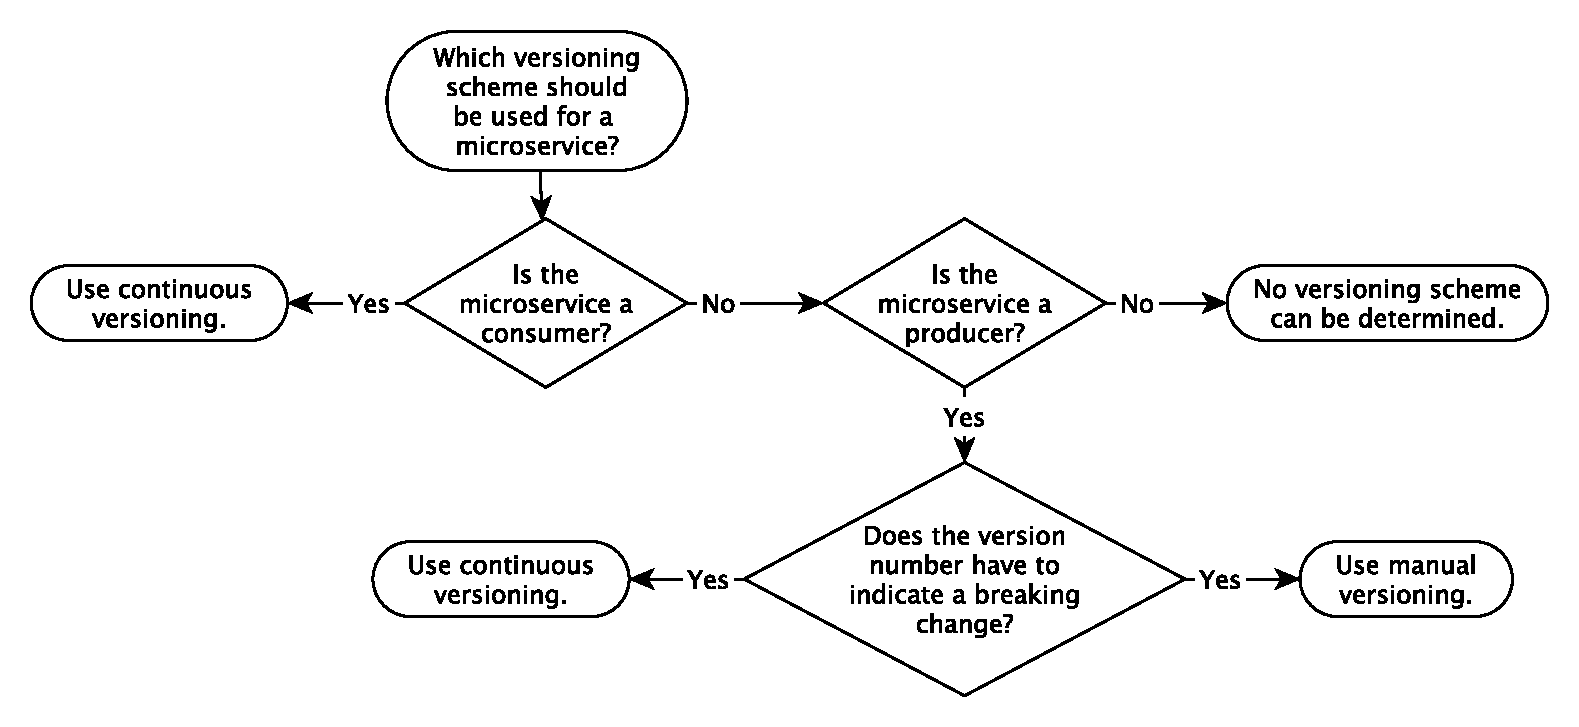
\includegraphics[scale=0.55]{images/figures/versioning_decision_flow.pdf}
\end{center}
\caption{A decision flow helping to select the best versioning scheme for a
microservice.}%
\label{fig:versioning_decision_flow}
\end{figure}


\subsection{Economic Benefits of Continuous Versioning}%
\label{sub:Economic_Benefits_of_Continuous_Versioning}
\ac{CI}/\ac{CD} systems already help developers by removing the need to
manually build and deploy their software. In addition, DevOps practises give
developers the ability to fully control their deployment infrastructure and
thus eliminating additional operations teams. Continuous versioning takes this
idea even further. Instead of development teams manually having to set a
version number, this process can now be federated to a \ac{CI} system. Only in
cases where the version number holds a semantic meaning (e.g.\ a break in
backward compatibility) a continuous versioning scheme can not be used. In the
end, another process that is being automated means more time that developers can
focus on the task of advancing the application's feature set and innovating.
Hence, not only the development teams benefits but also the company carrying it
out.
